\documentclass{article}
\usepackage[parfill]{parskip}
\usepackage[utf8]{inputenc}
\usepackage{amsmath}
\usepackage{amsthm} % for proofs
\usepackage{amssymb}
\usepackage{graphicx}
\usepackage{bm}
\usepackage[toc,page]{appendix}
\graphicspath{ {./images} }

\title{Homography}
\author{Dávid Iván}

\begin{document}

\maketitle

\tableofcontents

\newpage

\section{Vanishing point and distances}

How is the 3D distance related to the distance on the image taken by a pinhole camera? Consider the following figure.

\begin{figure}[ht]
 \centering
  \includegraphics[width=330pt]{images/camera_and_geometry.png}
 \caption{Camera geometry.}
\end{figure}

$C$ is the camera center. The red line crossing through $O$ and $A$, is an arbitrary line in 3D, that is not parallel to the image plane $\pi$. Consider $O$ as the origin on the red line, and as we slide $A$ on the line, $A'$ slides as well on the image plane. As $A$ tends to infinity, $A'$ tends to $P'_{\text{inf}}$. All the points marked on the figure are on one plane that can be seen on the next figure.

\begin{figure}[ht]
 \centering
  \includegraphics[width=330pt]{images/geometry.png}
 \caption{Plane geometry.}
\end{figure}

Point $B$ is the intersection of the image plane and the red line. Drawing a parallel line with $AC$ from $B$, intersects the line $CP'_{\text{inf}}$ at point $D$. Similarly, but parallel with $OC$ we get the point $E$. Thus $|DE| = |OA| \equiv x$.

Triangle $A'CP'_{\text{inf}}$ is similar to the triangle $BDP'_{\text{inf}}$:

\begin{equation} \label{eq:sim1}
    \frac{|A'P'_{\text{inf}}|}{|CP'_{\text{inf}}|} = \frac{|BP'_{\text{inf}}|}{|DP'_{\text{inf}}|}
\end{equation}

Triangle $O'CP'_{\text{inf}}$ is similar to the triangle $BEP'_{\text{inf}}$:

\begin{equation} \label{eq:sim2}
    \frac{|O'P'_{\text{inf}}|}{|CP'_{\text{inf}}|} = \frac{|BP'_{\text{inf}}|}{|EP'_{\text{inf}}|}
\end{equation}

Dividing (\ref{eq:sim1}) by (\ref{eq:sim2}) we get

\begin{equation}
    \frac{|A'P'_{\text{inf}}|}{|O'P'_{\text{inf}}|} = \frac{|EP'_{\text{inf}}|}{|DP'_{\text{inf}}|}
\end{equation}

Denote $|O'P'_{\text{inf}}| \equiv d'_{\inf}$, $O'A' \equiv x'$ and $EP'_{\text{inf}} \equiv \delta$.

With these we can write:

\begin{equation}
    \frac{d'_{\text{inf}} - x'}{d'_{\text{inf}}} = \frac{\delta}{\delta + x}
\end{equation}

From this we get:

\begin{equation} \label{eq:vanishing}
    \boxed{\frac{x'}{d'_{\text{inf}}} = \frac{x}{\delta + x}}
\end{equation}


Let's plot $x'/d'_{\text{inf}}$ against $x/\delta$:

\begin{figure}[ht]
 \centering
  \includegraphics[width=250pt]{images/projection_function.png}
 \caption{Plot.}
\end{figure}

\subsection{getting the vanishing point.}

Now assume that instead of having one point $A$ on the red line, we have $A_1$ and $A_2$ such that $|OA_1| = |A_1A_2| \equiv \Delta x$. (See figure)

\begin{figure}[ht]
 \centering
  \includegraphics[width=330pt]{images/vanishing_point.png}
 \caption{3D geometry for calculating the vanishing point.}
\end{figure}

Using (\ref{eq:vanishing}) we can write these equations:

\begin{equation}
    \frac{\Delta d_1}{d'_{\text{inf}}} = \frac{\Delta x}{\delta + \Delta x}
\end{equation}

\begin{equation}
    \frac{\Delta d_1 + \Delta d_2}{d'_{\text{inf}}} = \frac{2\Delta x}{\delta + 2\Delta x}
\end{equation}

From these we can derive a formula for the vanishing distance:

\begin{equation}\label{eq:vanishing_distance}
    \boxed{d'_{\text{inf}} = \frac{\Delta d_1 (\Delta d_1 + \Delta d_2)}{\Delta d_1 - \Delta d_2}}
\end{equation}

Note that we do not need to know $\Delta x$, the distances in 3D space, only the distances on the image ($\Delta d_1$, $\Delta d_2$).

\newpage
\subsection{application example}

Let's look at an example (look at the image below), where we have $\Delta d_1 = 57.55$, $\Delta d_2 = 32.25$. With these we can substitute into (\ref{eq:vanishing_distance})

\begin{equation}
    d'_{\text{inf}} = \frac{\Delta d_1 (\Delta d_1 + \Delta d_2)}{\Delta d_1 - \Delta d_2} = \frac{57.55 \cdot (57.55 + 32.25)}{57.55 - 32.25} = 204.27
\end{equation}

\begin{figure}[ht]
 \centering
  \includegraphics[width=250pt]{images/vanishing_point_example.png}
 \caption{Example of calculating the vanishing point position.}
\end{figure}


\end{document}